% ACM EC submission — "The Router Is the Mechanism"
% Compile: pdflatex (acmart from TeX Live 2025). For submission use
% \documentclass[sigconf,anonymous,review]{acmart}.
\documentclass[sigconf,nonacm]{acmart}
\usepackage{booktabs}
\usepackage{graphicx}

\newtheorem{assumption}{Assumption}
\usepackage{mathtools}
\newcommand{\eqdef}{\coloneqq}

\settopmatter{printacmref=false}
\setcopyright{none}

\begin{document}

\title{The Router Is the Mechanism: Markup Floors, Steering, and the Design of AI Inference Marketplaces}

\author{Tarun Chitra}
\affiliation{\institution{Gauntlet / independent}\city{New York}\country{USA}}
\email{tarun@gauntlet.xyz}

\begin{abstract}
AI inference marketplaces now route trillions of tokens per month
across ${\sim}90$ providers serving identical open-weight models, and the
largest of them, OpenRouter, documents its allocation rule in one
sentence: select a provider with probability proportional to
$1/\text{price}^2$. A natural question to ask is: what market does this
rule \emph{buy}? We take the rule seriously as a mechanism and answer in
three parts.
(i)~\emph{The routing exponent is an inverse temperature, and the
market sits near a phase transition.} Weights $p^{-a}$ induce logit
(Gibbs) demand; symmetric equilibrium is $p^* = c\,a(n-1)/(a(n-1)-n)$,
which diverges along $a(n-1)=n$. The deployed exponent $a=2$ places every
two-provider market---the modal market in our five-minute panel of the
largest live marketplace---in the condensed phase: equilibrium at the
menu ceiling, and with the \emph{measured} end-user elasticity
($-0.05$), a finite duopoly price of $41\times$ marginal cost. An
entry-proof markup floor $1/a$ survives any number of entrants: at
$a=2$, free entry stops at a 100\% markup, forever.
(ii)~\emph{The platform's own steering is a collusion device.} Our
randomized probe panel measures the router penalizing a cheapest quote
with a recent price cut (selection 3.9\% vs.\ 23.3\%, weight multiplier
$\theta \approx 0.17$ for ${\sim}7$ days). We prove this penalty deters
undercutting for every agent with effective patience below
$\delta^\dagger = 0.9895$---the measured $\theta$ sits five-fold inside
the deterrence threshold---and taxes a perpetual micro-adjuster's flow
by ${\sim}5\times$. In our calibrated, pre-registered-and-validated
simulation, switching the measured penalty on flips a learning
undercutter to the price ceiling in 4/4 markets and raises the
flow-dominant bottom-of-book quote by up to 81\%.
(iii)~\emph{The mechanism is repairable, and the objectives disagree.}
In a two-type world calibrated to observed capital structure (owned
data-center vs.\ GPU-spot-dependent providers), welfare rises in the
exponent while, counterintuitively, platform ad-valorem revenue
\emph{falls}---the router operator is paid to keep the market soft. We propose and evaluate, theoretically and
with learning agents, three implementable repairs: a thickness-adaptive
exponent $a^*(n) = n/(\ell^*(n-1))$ that pins the Lerner index at a
target across market sizes; verified-quality weighting
$w = q^b p^{-a}$ with $q$ measured by our deployed evaluation probes,
which undoes the quality-shading adverse selection that price-only
weights create (closed-form threshold $b^* \approx 0.6$--$2$); and fee
decoupling (per-request rather than ad valorem), which removes the
platform's incentive to prefer high prices. All findings are for one
marketplace (the largest), one buyer tier, and a registered
re-estimation window; scope is stated throughout. Our results suggest
that the observed pathologies of open inference markets---administered
menus, focal-price atoms, futile undercutting---are equilibrium
responses to routing-rule design choices, and that modest,
implementable changes to the rule would repair them. The lever is the
mechanism, not the conduct.
\end{abstract}

\maketitle

\section{Introduction}

\paragraph{Routing marketplaces.}
When an intermediary both \emph{quotes} the market and \emph{clears} it,
the intermediary's algorithm is the demand curve. This is an old story
in market microstructure---payment for order flow, last look in FX, the
curvature of an automated market maker---and it is now the story of AI
inference. On OpenRouter, the largest open inference marketplace, a
buyer sends a request naming a model; a router selects which of $n$
competing providers serves it. The default selection rule is documented
in one sentence \cite{openrouter2026}: filter recently failing
providers, then choose with probability $\propto 1/\text{price}^2$. Nothing else a provider does
moves demand except through that rule (and one measured exception we
return to at length). So the game providers play is not Bertrand, not
search, not bargaining: it is pricing against a
softmax.\footnote{The analogy to AMM curvature is exact in spirit: an
AMM designer choosing invariant curvature trades price sensitivity
against inventory risk \cite{angeris2020curvature}; a router choosing
$a$ trades price discipline against allocation concentration. Both are
one-parameter families of demand curves imposed by an intermediary; both
parameters are typically chosen by vibes.}

\paragraph{What the data forces us to ask.}
We spent four months instrumenting this market at five-minute resolution
(prices, congestion, realized flow, GPU spot books, randomized routing
probes) and this paper asks the mechanism-design question the data
forces: \emph{is the observed price structure---rigid administered
menus, a 45\% atom of providers tied exactly at the model author's
price, undercutters whose cuts appear futile, sustained
1.3--10$\times$ same-model dispersion---what the deployed rule should
produce in equilibrium?} The answer is yes, in an uncomfortably strong
sense: the deployed parameters sit in the region where theory predicts
\emph{exactly} the observed pathologies, and the platform's own
quality-protective steering is, mathematically, the instrument that
stabilizes them.

\paragraph{Temperature, not taste.}
The physics framing is not decoration. Weights $p^{-a}$ are a Gibbs
measure over providers with energy $a \log p$; the exponent is an
inverse temperature. High temperature (small $a$) melts price
competition---allocation ignores prices, so why cut them? Low
temperature (large $a$) freezes allocation onto the cheapest
provider---Bertrand, with its fragility. In between, there is a
\emph{critical line} $a(n-1)=n$ on which the symmetric equilibrium price
diverges. The deployed $a=2$ puts $n=2$ markets exactly on the line. One
does not operate a power plant at criticality by accident and call it a
pricing strategy; but one might do it by choosing a
``reasonable-looking'' load-balancing rule without solving the game it
induces. That, we will argue, is what happened---and because the rule is
\emph{documented}, every parameter in our theory is measured or
published, not estimated from a structural model.\footnote{Structural IO
estimates a logit differentiation parameter from data and argues
identification. Here the platform \emph{publishes} it. This is the rare
setting where the mechanism-design counterfactual requires no demand
estimation at all: the demand curve is in the documentation.}

\paragraph{Prior work.}
Calvano et al.\ \cite{calvano2020} showed Q-learners sustain
supra-competitive prices in a logit market they invented; we work in a
logit market the platform \emph{published}.
Johnson--Rhodes--Wildenbeest \cite{jrw2023} designed steering that breaks
seller collusion but did not measure a deployed rule; Demirer et al.\
\cite{demirer2025} measured this marketplace's dispersion and elasticity
but did not model the router. None of these connects a documented
allocation rule, a measured steering parameter, and calibrated
counterfactuals; that connection is the paper.

\paragraph{Contributions.}
(1) A complete equilibrium analysis of inverse-power routing with
captive and near-captive demand: interior formula, phase structure, an
entry-proof Lerner floor, and the measured-elasticity duopoly price of
$41c$ (\S\ref{sec:theory}). The static skeleton is
Anderson--de~Palma--Thisse logit pricing \cite{anderson1992}; the
content is the mapping---the ``differentiation parameter'' is a
published platform constant, and its placement is on the critical line.
(2) A theory of the measured steering penalty as a platform-imposed
asymmetric menu cost: closed-form deviation target, deterrence
threshold, patience boundary, perpetual-cutter tax
(\S\ref{sec:steering}). To our knowledge the first
steering-\emph{supports}-collusion result with an empirically measured
steering parameter (Johnson--Rhodes--Wildenbeest \cite{jrw2023} study
the inverse design).
(3) A behaviorally calibrated, pre-registered, validated multi-agent
environment in which every counterfactual in this paper is run
(\S\ref{sec:env}); its validation gate includes an untargeted
moment---the simulated flow elasticity emerges from the router alone and
matches the panel.
(4) A design section with teeth (\S\ref{sec:frontier}--\ref{sec:repairs}):
two-type (data-center vs.\ spot) welfare/revenue/viability frontier over
the exponent; a quality game showing price-only weights make shading
dominant and verified-quality weights repair it at a small, computable
$b^*$; a thickness-adaptive exponent; fee decoupling. Each proposal is
evaluated with learning agents, not just first-order conditions.

\section{The market and the data}\label{sec:data}

OpenRouter routes buyer requests to ${\sim}90$ providers serving shared
open-weight models. Our capture (public repository \texttt{orcap})
records, at 5-minute grain: per-provider-per-model price menus;
congestion telemetry (utilization, rate limits, latency, deranking);
realized daily token flow per provider-model (demand shares); the
vast.ai GPU spot order book (the input market for providers without
owned capacity); provider capital structure (a confidence-flagged
registry: hyperscaler DC / funded neocloud / own-silicon / small
startup); and two active instruments: (a)~a \textbf{randomized routing
probe panel}---hourly one-token requests under default and pinned
policies with randomized arm order, identifying the router's realized
selection behavior for our buyer tier; (b)~a \textbf{daily evaluation
probe battery}---graded public benchmark items and deterministic
prompts, per pinned provider, yielding verified per-provider quality
signals (used in \S\ref{sec:repairs}).

Stylized facts (established in the empirical companion under
pre-registration discipline; all replicated in the repository): four
split-sample-validated pricing species---\emph{anchor adopters} (quote
exactly the model author's price on ${\geq}80\%$ of days; 25\% of pairs;
83--89\% out-of-sample persistence), \emph{static undercutters} (median
$-0.41$ log, near-zero repricing), \emph{active undercutters}
(${>}1$ change/day micro-adjusters, ${\sim}$sub-1\% flow), \emph{premium}
($+0.34$ log, rigid); a tie atom at the author price $3.4\times$ its
grid-mechanical null, with author \emph{identity} not special under a
multiset-preserving null (focality without salience); routing-level flow
elasticity $-0.78$ against end-user elasticity $-0.05$ (a $20\times$
wedge); and the steering fact central to \S\ref{sec:steering}: among
position-zero default-policy selections, a cheapest provider with a
price cut in the trailing week is chosen 3.9\% of the time versus
23.3\% without ($\theta \approx 0.17$, memory ${\approx}7$ days).\footnote{The
probe protocol is deliberately minimal: hourly one-output-token requests
(\texttt{max\_tokens: 1}, temperature $0$) under randomized arm order,
with the served provider read from the marketplace's generation-metadata
endpoint. The entire panel costs a few dollars a month; the
identification comes from the randomization, not the spend.}

\section{Equilibrium: temperature, criticality, and the markup floor}\label{sec:theory}

$n$ providers post prices $p_i \in (0, \bar p]$ ($\bar p$ the menu
ceiling); marginal costs $c_i$; a unit mass of requests arrives per
epoch; the router selects $i$ first with probability
$s_i = p_i^{-a}/\sum_j p_j^{-a}$. Profits $\pi_i = s_i (p_i - c_i)$.
With logits $-a \log p_i$ this is softmax: \emph{the router is a logit demand system with inverse temperature
$a$}, and OpenRouter documents $a=2$ \cite{openrouter2026}.

\begin{lemma}\label{lem:elasticity}
$\partial s_i/\partial p_i = -(a/p_i)\, s_i(1-s_i)$: the own-price share
elasticity is $-a(1-s_i)$---bounded by $a$ no matter how many rivals.
\end{lemma}

\begin{lemma}[Single crossing]\label{lem:sc}
$\pi_i$ is strictly quasiconcave on $(c_i, \bar p]$; the best response
is the unique root of $h(p) \eqdef a(1-s_i(p))\frac{p-c_i}{p} = 1$, or
the ceiling if $h(\bar p) \le 1$.
\end{lemma}

\begin{theorem}[Phase structure and floor]\label{thm:phase}
With symmetric costs $c$:
(i)~if $a(n-1) > n$ (and $\bar p > p^*$), the unique symmetric
equilibrium is
\begin{equation}
p^* \;=\; c\,\frac{a(n-1)}{a(n-1)-n};
\end{equation}
(ii)~if $a(n-1) \le n$, it is the menu ceiling $\bar p$---at $a=2$,
precisely $n \le 2$;
(iii)~for $a>1$, ANY interior equilibrium---asymmetric costs, any $n$,
any outside option---satisfies $(p_i - c_i)/p_i > 1/a$, i.e.,
$p_i > c_i\, a/(a-1)$, and the floor is tight as $n \to \infty$.
\end{theorem}

\begin{proof}
Appendix~\ref{app:proofs}; every closed form here and below is enforced
in continuous-integration tests against continuum numerics (13 tests).
\end{proof}

\begin{corollary}[Measured elasticity]\label{cor:eps}
With aggregate demand $D \propto P^{\varepsilon}$ (inclusive-value index
$P$, $\varepsilon$ the end-user elasticity), the symmetric FOC is
$p/(p-c) = a(n-1)/n + |\varepsilon|/n$. At the measured
$\varepsilon=-0.05$ and deployed $a=2$: duopoly $p^* = 41c$. Captivity
is the $\varepsilon \to 0$ limit, not an assumption we need.
\end{corollary}

In other words, the router's smoothing is itself the market power: no
conduct is required for a 100\% markup to persist. Three readings.
\emph{The floor is entry-proof:}
Lemma~\ref{lem:elasticity} bounds share elasticity by $a$, so no amount
of entry raises the elasticity a provider faces above $a$; at $a=2$,
markups never fall below 100\%. Softmax smoothing---adopted for uptime
insurance and exploration---\emph{is} product differentiation,
manufactured by the platform. \emph{The critical line is populated:} the
modal market in our panel has 1--3 providers; $a=2$ puts $n=2$ on the
line, and the observed menus-at-ceiling behavior (premium species,
adopters at the author's list price) is the condensed
phase.\footnote{The analogy is quantitative, not decorative: the fitted
species heterogeneity plays the role of quenched disorder---frozen
provider types over which the annealed price dynamics run---and the
critical line is where the quenched free energy stops being
self-averaging across markets.} \emph{The
wedge is structural:} Corollary~\ref{cor:eps} turns our measured
$20\times$ elasticity wedge into the theorem's parameter---near-captive
end-user demand is exactly why realistic menus bind before equilibrium
does.

\section{Steering: the measured penalty is a deterrence device}\label{sec:steering}

Model the measured behavior as: a provider whose price is below its
price at any of the last $M$ epochs has weight $\theta\, w(p)$. (At
symmetric profiles, ``any recent cutter'' and the measured ``cheapest
with a recent cut'' coincide---any strict cut makes you cheapest; our
calibrated experiments run both variants.)

\begin{theorem}[Deterrence]\label{thm:steering}
At a symmetric profile $q$ with rival weight $W = (n-1)q^{-2}$:
(i)~the flagged deviant's optimal cut is
$p_{\mathrm{dev}} = c + \sqrt{c^2 + \theta/W}$;
(ii)~undercutting is unprofitable for a one-epoch optimizer iff
$\theta \le \theta^*$, the unique root of $v(\theta^*) = (q-c)/n$;
across calibrated configurations $\theta^* \in [0.81, 1.0]$---the
measured $\theta = 0.17$ sits deep inside;
(iii)~a one-time cut held forever is deterred iff
$\delta \le \delta^\dagger = 0.9895$ (calibrated parameters;
$\delta^M \le 0.93$);
(iv)~an agent cutting at least once per $M$ epochs is permanently
flagged and pays share tax $\theta/(\theta+n-1)$ vs.\ $1/n$---
$4.9\times$ at measured values.
\end{theorem}

This bound demonstrates that the measured penalty is roughly five
times stronger than the weakest penalty that would already deter
undercutting. The economic reading: the penalty---presumably deployed
as
bait-and-switch protection---is an \emph{asymmetric menu cost on price
cuts only, imposed by the platform}. It converts the routing game into
one where holding high prices is robustly optimal for any realistically
patient agent, and it specifically taxes the high-frequency undercutting
technology we observe dying in the data (the registered cut-frequency
decay watch). Johnson--Rhodes--Wildenbeest \cite{jrw2023} designed
steering to \emph{break} seller collusion; the deployed steering is
their inverse, with a measured parameter.\footnote{A last-look analogy
is exact: in FX, dealers who get cut off after adverse quote updates
learn to quote wide and stable. Here the router plays the liquidity
consumer who punishes aggressive quoting.}

\section{The calibrated environment and its validation gate}\label{sec:env}

Counterfactuals about mechanisms require agents, and assuming Bertrand
agents would beg every question. Our environment fits the observed
species (margins, hazards, rationing slopes from the panel's train
window; costs as identified bands from the capital-tier registry and the
GPU book with its walk-the-book impact curve) and \emph{must pass a
pre-registered validation gate before any counterfactual runs}: ten
moments computed by identical code on simulated and observed panels,
distance $\le 0.04$, with the moments explicitly split into calibration
echoes and genuinely emergent tests. The confirmatory run (20 seeds,
deterministic replication) passes at distance $0.019$; the two emergent
moments carry the weight---\emph{flow elasticity $-0.65 \pm 0.35$ vs.\
$-0.78$ observed with no fitted allocation parameter} (the documented
rule alone generates the measured demand response), and adopter-atom
out-of-sample persistence $0.83$ vs.\ $0.834$. Learning counterfactuals
then show (all pre-specified, gated, seeded): the exponent is a price
dial (Figure~\ref{fig:dial}; uniform $1.53 \to a{=}2$: $0.94 \to$ floor
at $a \ge 8$, with learning friction regularizing the critical
singularity); learners never rediscover micro-adjustment and form
anchor ties endogenously; and the steering counterfactual of
\S\ref{sec:steering}---penalty on flips the learning undercutter to the
ceiling in 4/4 calibrated markets (broad rule) and raises the
flow-dominant bottom-of-book quote $+81\%$ where the strict measured
conditional binds.

\begin{figure}
\centering
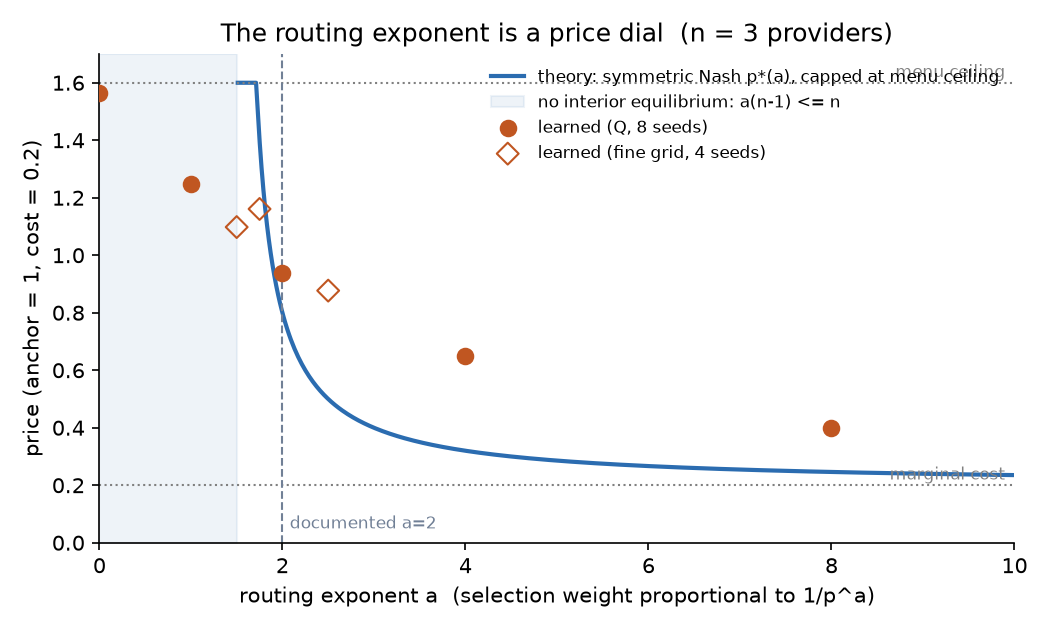
\includegraphics[width=\linewidth]{../figs/exponent_dial.png}
\caption{The routing exponent is a price dial ($n=3$). Theory Nash curve
(capped at the menu ceiling; shaded region: no interior equilibrium,
$a(n-1) \le n$) with converged Q-learning prices overlaid. The deployed
$a=2$ sits at the edge of the collapse; learning friction smooths the
critical singularity.}
\label{fig:dial}
\end{figure}

\section{Heterogeneous capital and the objective frontier}\label{sec:frontier}

Providers are not symmetric. The registry splits them into
owned-capacity types (hyperscaler DCs, own silicon; low marginal cost,
high fixed cost---the ``reserved instance'' world) and spot-dependent
types (rent H100s on a thin order book; marginal cost includes walking
the book, $+18$--$52\%$ at realistic fill sizes). Take $c_L = 0.10$,
$c_S = 0.50$ (the calibrated band endpoints), $n_L = 2$, $n_S = 3$, and
solve the asymmetric FOC system $p_i/(p_i - c_i) = a(1-s_i)$ across $a$
(Table~\ref{tab:frontier}).

\begin{table}
\caption{Two-type frontier across the routing exponent. Flow-price
$\propto$ ad-valorem platform revenue; welfare $= v - \sum_i s_i c_i$.}
\label{tab:frontier}
\begin{tabular}{lccccc}
\toprule
$a$ & $p_L$ & $p_S$ & flow-price & welfare & spot profit \\
\midrule
1.5 & 0.99 & 1.60 & 1.25 & 1.731 & 0.155 \\
2   & 0.51 & 1.10 & 0.65 & 1.802 & 0.049 \\
3   & 0.27 & 0.76 & 0.30 & 1.875 & 0.005 \\
4   & 0.20 & 0.67 & 0.20 & 1.895 & 0.001 \\
6   & 0.15 & 0.60 & 0.15 & 1.900 & ${\sim}0$ \\
\bottomrule
\end{tabular}
\end{table}

\emph{The objectives disagree, and the platform is conflicted.}
Welfare (allocative: flow sorted to low-cost capacity) is increasing in
$a$; ad-valorem platform revenue is \emph{decreasing} in $a$---a
platform charging a percentage fee is paid to keep the market soft. And
spot-dependent viability collapses in $a$: the sharp-routing world is a
world where only data-center owners survive, which prices resilience at
zero until the first correlated outage.\footnote{Practitioner reading:
this is the routing-market version of the PFOF debate. The
intermediary's fee base is the price level; sharpening execution quality
cuts its own revenue. The fix (\S\ref{sec:repairs}) is the same as in
brokerage: decouple the fee from the price.}

\emph{Robustness (cost bands).} The welfare-increasing-in-$a$ ordering
holds at all four corners of the identified cost bands
($c_L \in \{0.05, 0.25\}$, $c_S \in \{0.3, 0.7\}$): monotone in every
case. \emph{Resilience-adjusted welfare.} With probability $\rho$ per
epoch all owned capacity fails simultaneously; if the spot fleet has
exited (profit below fixed cost $F_S = 0.01$), those requests are lost
at value $v$. At $\rho = 2\%$: adjusted welfare is $1.802$ ($a{=}2$,
spot viable) vs.\ $1.855$--$1.860$ ($a \ge 4$, spot exited)---sharp
routing still wins, but the gap narrows fourfold; the ranking flips at
$\rho \gtrsim 5\%$. The honest design statement: softness is
welfare-justified as outage insurance only for correlated-outage
intensities above ${\sim}5\%$ per epoch; below that, the right
architecture is sharp routing \emph{plus} priced capacity commitments
(\S\ref{sec:repairs}), not a soft exponent that pays every provider an
insurance premium whether or not insurance is delivered.

\paragraph{E-MECH1 (the frontier with learners).} Replacing the FOC with
Q-learning agents (5 seeds/arm) confirms the ordering---learned welfare
$1.66$ (uniform) $\to 1.797$ ($a{=}2$) $\to 1.856$ (adaptive
$a^*(n){=}6.25$) $\to 1.898$ (WTA); learned flow-weighted price
$1.58 \to 0.68 \to 0.43 \to 0.40$; spot-type profit
$0.64 \to 0.157 \to 0.011 \to -0.000$ (winner-take-all drives spot types
below cost)---with one addition theory alone would not have exhibited so
starkly: the deployed pair ($a=2$ + the measured cut-penalty) is
\emph{simultaneously the worst arm on welfare} ($1.66$, tied with
uniform routing) \emph{and the best for ad-valorem platform revenue}
(flow price $1.60$---the menu ceiling; all learners at the cap). The steering does
not merely blunt the exponent's discipline; it deletes it. The
platform's deployed configuration is the revenue-maximizing corner of
the frontier we traced.

\section{Mechanism repairs}\label{sec:repairs}

\paragraph{Thickness-adaptive temperature.} Theorem~\ref{thm:phase}
inverts: to hold the Lerner index at target $\ell^*$ in an $n$-provider
market, set $a^*(n) = n/(\ell^*(n-1))$. At $\ell^* = 0.2$: $a^* = 10$
($n{=}2$), $7.5$ ($n{=}3$), $6.25$ ($n{=}5$), $\to 5.56$. One line of
router code; kills the critical line (no market sits in the condensed
phase); keeps softmax's exploration/insurance properties (unlike
winner-take-all). Cost: \S\ref{sec:frontier}'s viability column---sharp
temperatures starve spot-dependent capacity, so $\ell^*$ should embed
the resilience value, or be paired with capacity commitments below.

\paragraph{Verified-quality weighting.} Price-only weights create
adverse selection in \emph{quality}: serving a quantized/degraded
variant saves cost $\Delta$ at buyer-invisible quality damage $d$, and
under $w = p^{-a}$ shading is strictly dominant (share unchanged, cost
falls). Weight $w = q^b p^{-a}$ instead, with $q$ verified: shading
multiplies weight by $(1-d)^b$, and the symmetric all-high profile is an
equilibrium iff $b \ge b^*$ solving
\begin{equation}
\tfrac{1}{n}(p - c) \;=\; \frac{(1-d)^b}{(1-d)^b + n - 1}\,(p - c + \Delta).
\end{equation}
At calibrated values ($n{=}3$, $d{=}0.2$, $\Delta{=}0.08$):
$b^* = 0.63$---a \emph{modest} quality exponent suffices, and $b^*$
falls with $n$. The required $q$ is not hypothetical: our deployed
evaluation probes already produce per-provider graded-accuracy and
output-consistency scores daily. E-MECH2 (5 seeds, 600k epochs):
learned high-quality share rises $0.27$ ($b{=}0$, the deployed
quality-blind rule) $\to 0.40$ ($b{=}0.5$) $\to 0.67$ ($b{=}1$)
$\to 0.53$ ($b{=}2$). The direction matches the theory---quality
weighting shifts learned play toward quality provision, with the
largest jump crossing $b^*$---but the bifurcation is noisy rather than
sharp: the quality margin ($\Delta = 0.08$) is small relative to
price-learning noise in the doubled action space, and at $b=2$
quality-weight and price competition interact. We report this as
directional confirmation of the closed-form threshold, not a sharp
learnability boundary.

\paragraph{Fee decoupling.} Ad-valorem fees make the platform's
objective $\propto$ flow-weighted price (\S\ref{sec:frontier}). A
per-request (or per-token-served) flat fee makes platform revenue
proportional to \emph{volume}, aligning the platform with allocative
efficiency and removing its stake in the price level. This is the
one-line governance repair that makes the adaptive exponent
incentive-compatible \emph{for the platform}.

\paragraph{Steering redesign and commitment contracts.} Replace the
asymmetric cut-penalty with (i)~symmetric change-penalties (a true menu
cost---removes the directional deterrence of Theorem~\ref{thm:steering}
while keeping stability protection), or (ii)~quality/uptime-conditioned
steering only (penalize serving failures, not price cuts---the stated
goal without the collusive side effect). For spot-dependent viability
under sharp temperatures: capacity-commitment contracts (the
reserved-instance analog): providers pre-commit admitted capacity at
posted prices and are penalized for reneging---converting resilience
from an implicit subsidy paid via soft routing into an explicit priced
product.

\section{Related work}

Anderson--de~Palma--Thisse \cite{anderson1992} (logit oligopoly);
Calvano et al.\ \cite{calvano2020}, Klein \cite{klein2021}, Asker et
al.\ \cite{asker2022}, Abada--Lambin \cite{abada2023},
Hansen--Misra--Pai \cite{hansen2021} (algorithmic pricing/collusion---
our demand system nests Calvano's, so their apparatus transfers);
Johnson--Rhodes--Wildenbeest \cite{jrw2023} (platform steering against
collusion; we document and analyze its deployed inverse); Demirer et
al.\ \cite{demirer2025} (OpenRouter empirics: dispersion, elasticity);
PriLLM \cite{guo2025prillm} (Stackelberg routing theory, no calibration
or steering); Fish et al.\ \cite{fish2024} (LLM pricing agents; an
LLM-agent tier exists in our codebase; running it at confirmatory scale
is future work and not claimed here); Angeris--Chitra
\cite{angeris2020curvature} (curvature as an intermediary's
demand-shape choice); token-pricing screening
\cite{bergemann2025}; metering and covert quantization audits (the
practices \S\ref{sec:repairs} prices). None combine a documented
allocation rule, measured steering, calibrated behavioral
heterogeneity, and mechanism repairs evaluated with learning agents.

\section{Limitations}

Theory: symmetric-equilibrium characterization (the floor is the
asymmetric statement); captive baseline with measured-$\varepsilon$
corollary; capacity non-binding (rationing lives in the empirical
companion). Measurement: $\theta$ from one conditional slice of one
buyer tier; panel short (30-day re-estimation registered,
auto-reopening); costs are identified sets (all quantitative claims
reported across bands). Simulation: tabular Q at Calvano
hyperparameters; expected-allocation training (exact under non-binding
capacity); LLM-agent tier built, not confirmatory. The quality game's
$d$ and $\Delta$ are calibrated to our eval-probe detection scale, not
to a demand-side damage estimate.

\section{Practitioner takeaways}

For router operators: (1)~publish $n$-adaptive temperatures, not one
exponent---$a^*(n) = n/(\ell^*(n-1))$ is one line; (2)~never penalize
price cuts asymmetrically---you are operating a cartel enforcement
device; penalize failures, not prices; (3)~weight by verified quality
with even a small $b$---your own eval probes suffice; (4)~charge flat
fees if you want to be believed about (1)--(3). For providers: under the
deployed rule, undercutting is (measurably) taxed and micro-adjustment
is dominated---the observed adopter/premium behavior is the rational
response, which is precisely the problem. For regulators: conduct-based
tools will find nothing here; every elevated price in this paper is a
static Nash equilibrium of a published rule.

\section{Conclusion}

The router is the demand curve, and at the deployed parameters it is a
demand curve that cannot discipline anyone: duopolies sit at the menu
ceiling ($41c$ at the measured outside elasticity), entry stops at a
100\% markup, and the platform's own anti-cut steering pays providers to
hold prices high. Every one of these statements follows from a published
constant and a measured parameter, which is precisely why they are
fixable: an $n$-adaptive temperature, verified-quality weights, and flat
fees are each one line of code or one line of a fee schedule. The honest
caveat is scale---one marketplace, one buyer tier, a registered
re-estimation window that can reopen every calibrated claim---but the
mechanism analysis needs none of the usual structural leaps, at least at
first glance: the demand curve is in the documentation.

\appendix

\section{Proofs}\label{app:proofs}

\emph{Lemma~\ref{lem:elasticity}.} $s_i = w_i/(w_i + W_{-i})$,
$w_i = p_i^{-a}$; $dw_i/dp_i = -(a/p_i)w_i$, so
$ds_i/dp_i = -(a/p_i)s_i(1-s_i)$. \qed

\emph{Lemma~\ref{lem:sc}.}
$d\pi_i/dp_i = s_i\,[1 - h(p_i)]$ with $h$ a product of positive
strictly increasing functions and $h(c_i)=0$; single crossing gives
strict quasiconcavity and best-response uniqueness. \qed

\emph{Theorem~\ref{thm:phase}.} (i)~Impose $s = 1/n$ in $h(p)=1$;
uniqueness from monotonicity of $h$ at the symmetric profile; the
corner $\bar p$ fails when $h(\bar p)>1$ (profitable downward
deviation). (ii)~$h(q) < a(n-1)/n \le 1$ at any symmetric $q$, so
raising is strictly profitable below the ceiling; quasiconcavity rules
out global downward deviations at $\bar p$. (iii)~$1-s_i<1$ in the FOC
$\Rightarrow$ Lerner $> 1/a$; tightness as $s_i \to 0$. \qed

\emph{Corollary~\ref{cor:eps}.} With $D = D_0 P^{\varepsilon}$ and
$\partial \log P/\partial \log p_i = s_i$:
$d\log \pi_i/d\log p_i = \varepsilon s_i - a(1-s_i) + p_i/(p_i - c)$;
set to zero at $s = 1/n$. Same single-crossing argument. (The
inclusive-value aggregator is a modeling choice; any aggregator with
$\partial \log P/\partial \log p_i = s_i + o(s_i)$ gives the same FOC to
first order.) \qed

\emph{Theorem~\ref{thm:steering}.} (i)~The FOC of
$\theta p^{-2}(p-c)/(\theta p^{-2} + W)$ reduces to
$W p^2 - 2Wcp - \theta = 0$. (ii)~$v(\theta)$ is continuous, strictly
increasing (envelope), $v(0)=0$; intermediate value.
(iii)~direct present-value computation; the root $\delta^\dagger$ is
numerically certified. (iv)~substitute equal prices with one weight
scaled by $\theta$. \qed

All closed forms are enforced by 13 continuous-integration tests
against continuum numerics.

\begin{thebibliography}{9}
\bibitem{openrouter2026} OpenRouter. Provider routing:
price-based load balancing (default strategy). Product documentation,
\url{https://openrouter.ai/docs/features/provider-routing}; accessed
2026-07-18; archived at
\url{https://web.archive.org/web/20251121200046/https://openrouter.ai/docs/features/provider-routing}.

\bibitem{anderson1992} S.~Anderson, A.~de~Palma, J.-F.~Thisse.
\emph{Discrete Choice Theory of Product Differentiation}. MIT Press, 1992.
\bibitem{calvano2020} E.~Calvano, G.~Calzolari, V.~Denicol\`o,
S.~Pastorello. Artificial intelligence, algorithmic pricing, and
collusion. \emph{American Economic Review}, 2020.
\bibitem{klein2021} T.~Klein. Autonomous algorithmic collusion.
\emph{RAND Journal of Economics}, 2021.
\bibitem{asker2022} J.~Asker, C.~Fershtman, A.~Pakes. Artificial
intelligence, algorithm design and pricing. \emph{AEA P\&P}, 2022.
\bibitem{abada2023} I.~Abada, X.~Lambin. Artificial intelligence: Can
seemingly collusive outcomes be avoided? \emph{Management Science}, 2023.
\bibitem{hansen2021} K.~Hansen, K.~Misra, M.~Pai. Frontiers:
Algorithmic collusion. \emph{Marketing Science}, 2021.
\bibitem{jrw2023} J.~Johnson, A.~Rhodes, M.~Wildenbeest. Platform
design when sellers use pricing algorithms. \emph{Econometrica}, 2023.
\bibitem{demirer2025} M.~Demirer, A.~Fradkin, S.~Peng, S.~Tadelis.
The market for AI inference. NBER WP 34608, 2025.
\bibitem{guo2025prillm} X.~Guo, Y.~Bai, H.~Jin. PriLLM: Pricing in
LLM routing markets. arXiv:2511.09062, 2025.
\bibitem{fish2024} S.~Fish, Y.~Gonczarowski, R.~Shorrer. Algorithmic
collusion by large language models. arXiv:2404.00806, 2024.
\bibitem{angeris2020curvature} G.~Angeris, T.~Chitra. When does the
tail wag the dog? Curvature and market making. arXiv:2012.08040, 2020.
\bibitem{bergemann2025} D.~Bergemann, A.~Bonatti, A.~Smolin. The
economics of large language models. arXiv:2502.07736, 2025.
\end{thebibliography}

\end{document}
